%\setdigitfont{Times New Roman}
%\setlatintextfont[Scale=1.2]{Times New Roman}
\chapter{پیاده\nf سازی در مقیاس کوچک بر روی سکوی مجازی\nf سازی}
\label{cwaio}
\setlatintextfont{Times New Roman}
\section{نصب}
برای پیاده\nf سازی به این روش، نیاز داریم فایل \lr{OVF} را که برای این نوع نصب بر روی سکوی مجازی\nf سازی ارائه شده است، در اختیار داشته\nf باشیم.  این فایل را می\nf توان از قسمت مربوط به نصب  بر روی سکّوی مجازی\nf سازیِ وب\nf سایت پروژه \href{http://projectclearwater.org}{\lr{clearwater}} و یا از طریق لینک زیر دانلود کرد. 

\begin{latin}
\setlength{\parindent}{0ex}
\href{http://vm-images.cw-ngv.com/cw-aio.ova}{\textcolor{blue}{http://vm-images.cw-ngv.com/cw-aio.ova}}
\end{latin}

برای نصب بر روی \lr{Virtualbox}، ابتدا این نرم\nf افزار را بازکرده و سپس از منوی \lr{\textbf{File}}، گزینه\nf ی \lr{\textbf{Import Appliance}}\RTLfootnote{\lr{Appliance} در واقع یک \lr{image} ماشین مجازی است که از قبل پیکربندی شده است.} را انتخاب کنید(شکل\ref{importApp}). راه\nf حل مشکلات احتمالی در نصب و پیکربندی \lr{VirtualBox} در پیوست (\ref{vboxA})  آورده شده است.

% همچنین، اگر تنظیمات کلیدهای میانبر این برنامه روی حالت پیش\nf فرض خود قرار داشته باشد، می\nf توان با فشردن دکمه\nf های ترکیبی \lr{\textbf{Ctrl+I}}، وارد این قسمت شد. 
\begin{figure}[H]
\centering
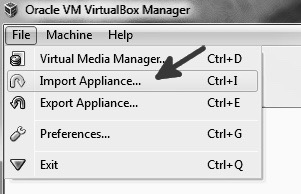
\includegraphics[width=0.5\textwidth]{importApp}
\caption{\lr{Import Appliance}}
\label{importApp}
\end{figure}
در پنجره بازشده، نواری وجود دارد که با کلیک بر روی آن، می\nf توان فایل موردنظر را انتخاب کرد. سپس بر روی دکمه \lr{\textbf{Next}}، کلیک کنید. در صفحه جدید، می\nf توانید تنظیمات مربوطه را مشاهده کنید. با کلیک بر روی گزینه \lr{\textbf{Import}}، عملیات نصب به\nf طور خودکار انجام می\nf شود(شکل\ref{importOVF}). در صورت وجود مشکل در ایجاد و اجرای ماشین مجازی، به پیوست (\ref{vboxAA}) مراجعه شود.

\begin{figure}[H]
\centering
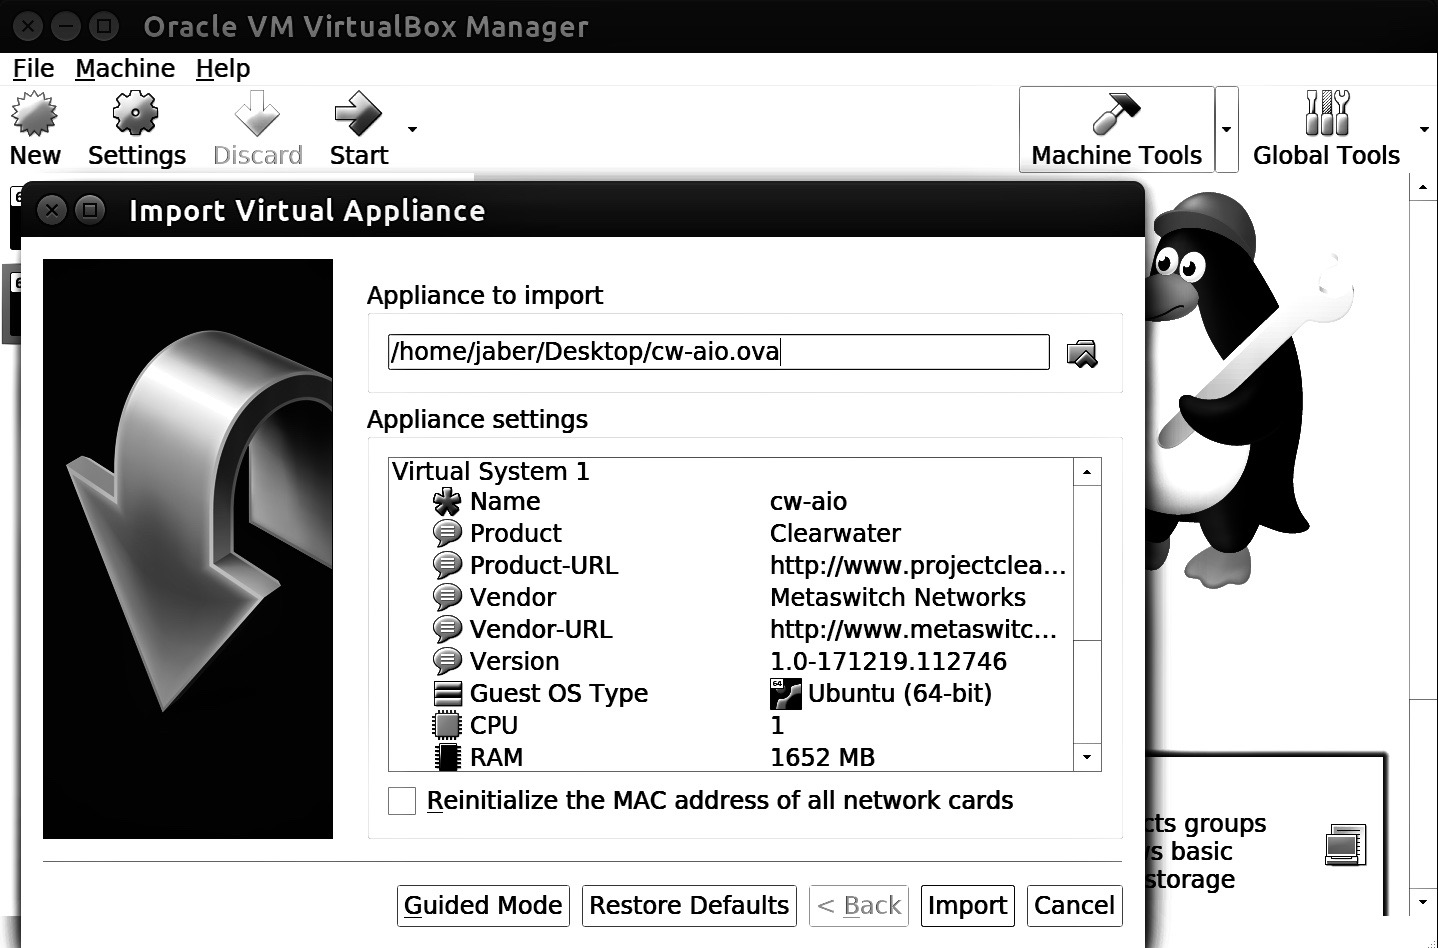
\includegraphics[width=0.5\textwidth]{importOVF}
\caption{\lr{Import OVF file}}
\label{importOVF}
\end{figure}

\section{راه\nf اندازی ماشین مجازی و ایجاد شماره تلفن}
پس از اتمام نصب، یک ماشین مجازی به نام \lr{cw-aio} به لیست ماشین\nf های مجازی نصب\nf شده بر روی \lr{Virtualbox} شما اضافه می\nf شود. با کلیک بر روی آن، ماشین مجازی \lr{clearwater} شروع به کار می\nf کند. پس از بالا آمدن صفحه ورود، از شما خواسته\nf می\nf شود که نام\nf کاربری و رمزعبور را وارد کنید. نام\nf کاربری  \lr{\textcolor{black}{'ubuntu'}} و رمزعبور \lr{\textcolor{black}{'cw-aio'}} است.


پس از ورود، از طریق ماشین میزبان یک مرورگر را به دلخواه باز کرده و در قسمت URL آن، عبارت  \href{http://localhost:8080}{\lr{\textcolor{blue}{http://localhost:8080}}} را وارد کنید. با انجام این کار، وارد صفحه\nf ای مشابه شکل \ref{ellisLogin} می\nf شوید. 
\begin{figure}[H]
\centering
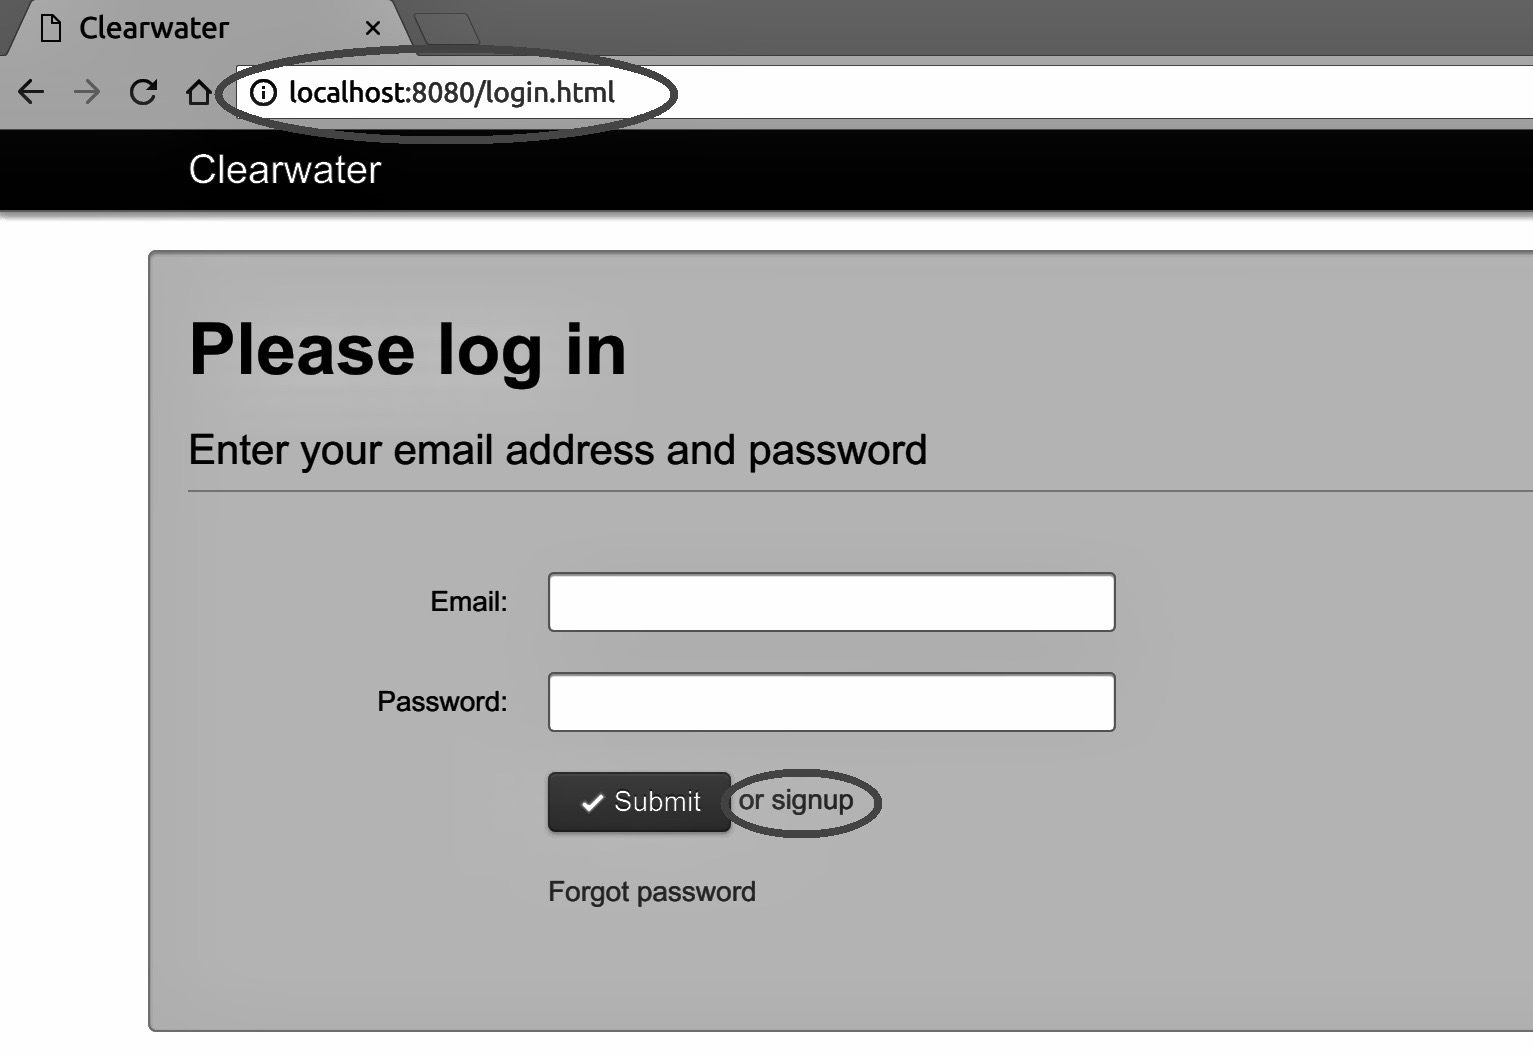
\includegraphics[width=0.5\textwidth]{ellisLogin}
\caption{صفحه\nf ی ورود}
\label{ellisLogin}
\end{figure}
در صورت عدم دسترسی به صفحه\nf ی وب، باید در قسمت \lr{URL}، عبارت \lr{<IP address>:8080} را وارد کنید و به جای عبارت \lr{<IP address>}، آدرس \lr{IP} ماشین میزبان را وارد کنید. لازم به ذکر است که پس از اجرای ماشین مجازی، باید اندکی صبر کنید تا سرور مربوطه شروع به کار کند و صفحه\nf ی مذکور، در دسترس شما قرار گیرد. 

 با ورود به این صفحه می\nf توان از طریق رابط کاربری وب، مشترکان پیاده\nf سازی clearwater  را مدیریت کرد. در صفحه\nf ای که وارد آن شده\nf اید، بر روی گزینه \lr{\textbf{signup}} کلیک کنید (اگر قبلاً ثبت\nf نام نکرده\nf اید). در صفحه\nf ی ثبت\nf نام(شکل\ref{signup})، اطّلاعات خواسته\nf شده ( نام، آدرس ایمیل و رمزعبور) را وارد کنید. اگر تیک گزینه \lr{\textbf{Demo Account}} را بزنید، انقضای حساب کاربری ساخته\nf شده پس از یک هفته تمام می\nf شود. در قسمت \lr{\textbf{signup code}}، عبارت \textcolor{black}{'secret'} را وارد کنید. در آخر، با کلیک بر روی دکمه \lr{\textbf{signup}}، حساب کاربری شما ساخته شده و وارد صفحه مربوط به مدیریت مشترکان می\nf شوید(شکل\ref{user}).

\begin{figure}[h]
\centering
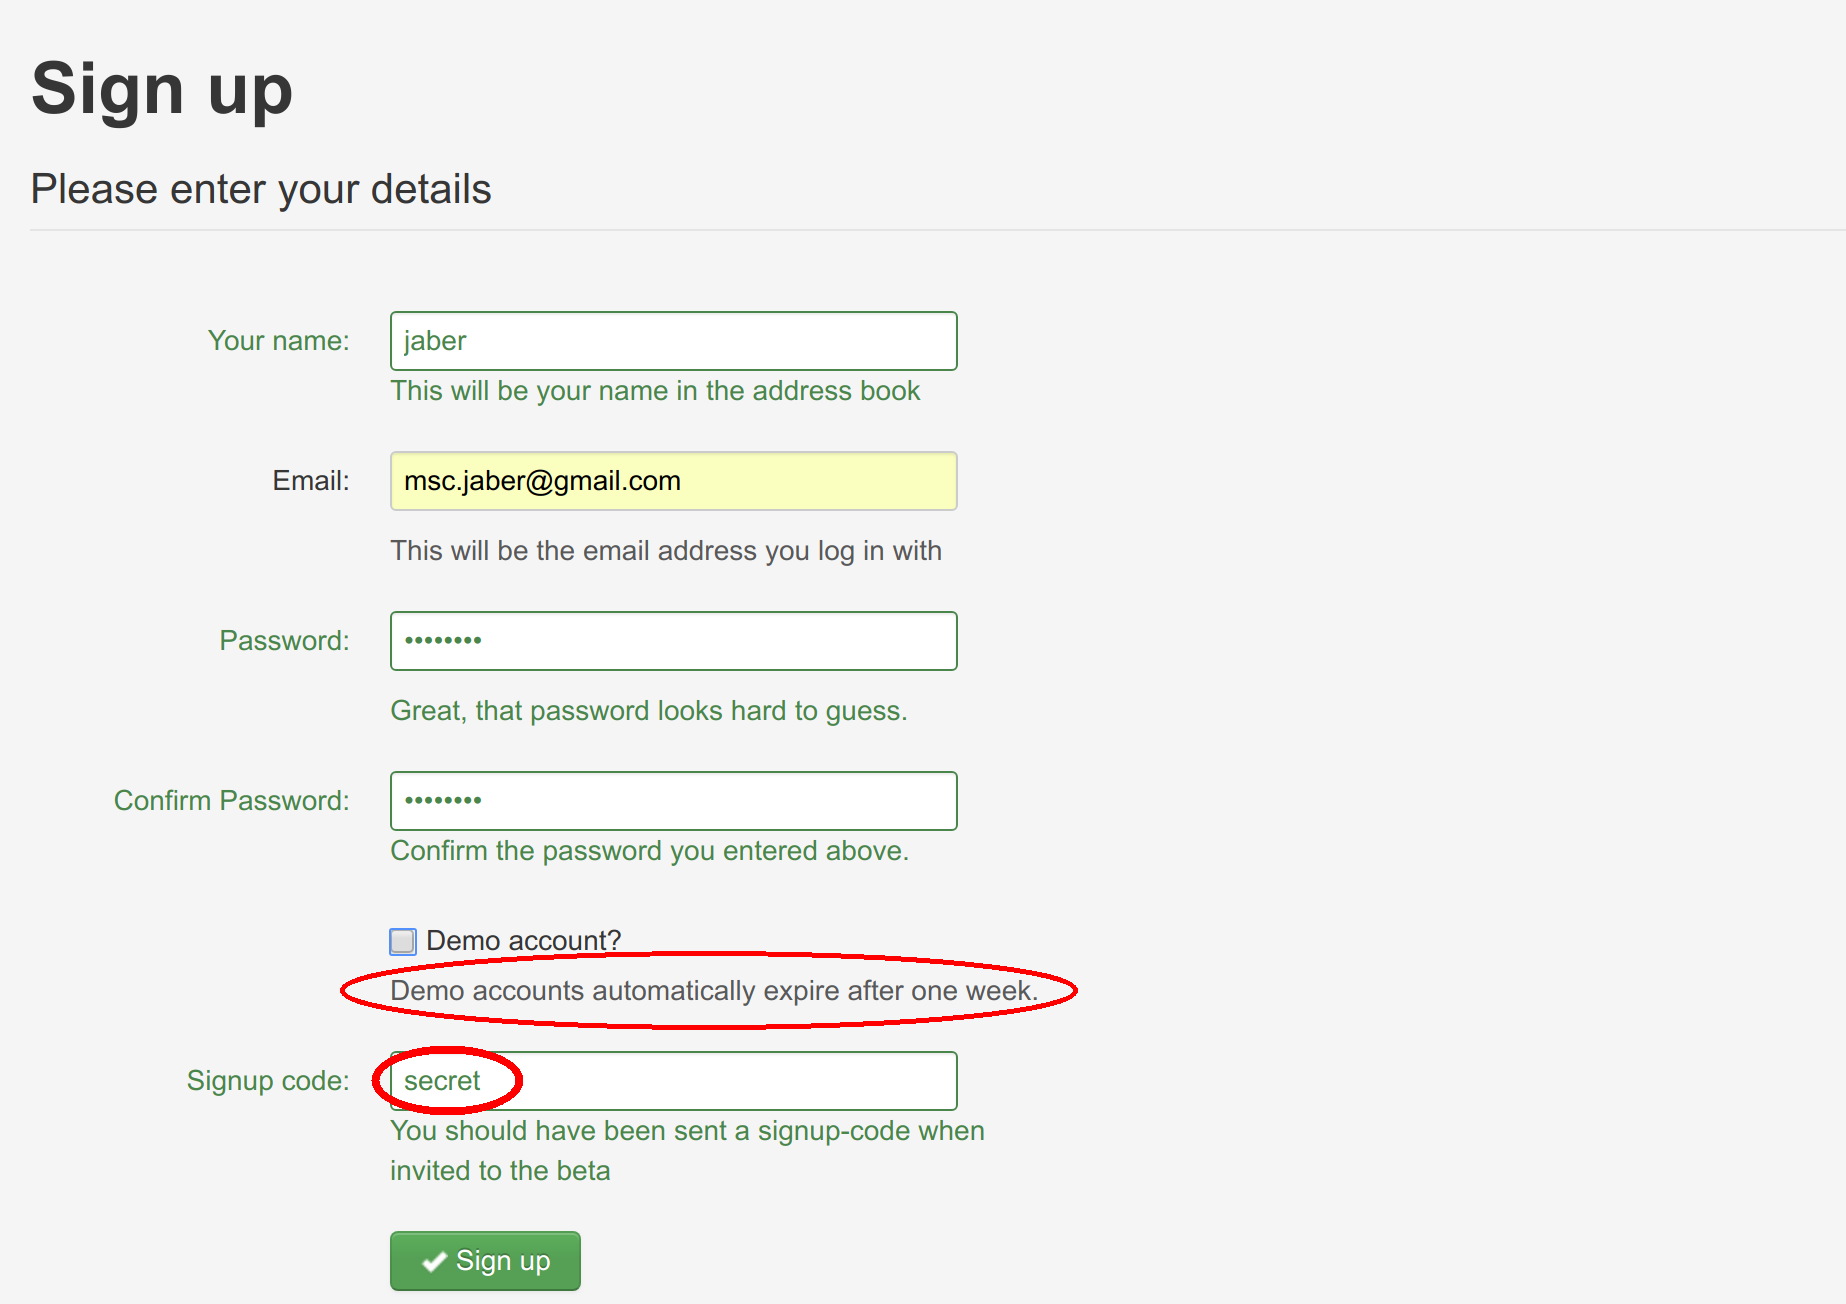
\includegraphics[width=\textwidth]{signup}
\caption{\lr{ثبت\nf نام}}
\label{signup}
\end{figure}


\begin{figure}[H]
\centering
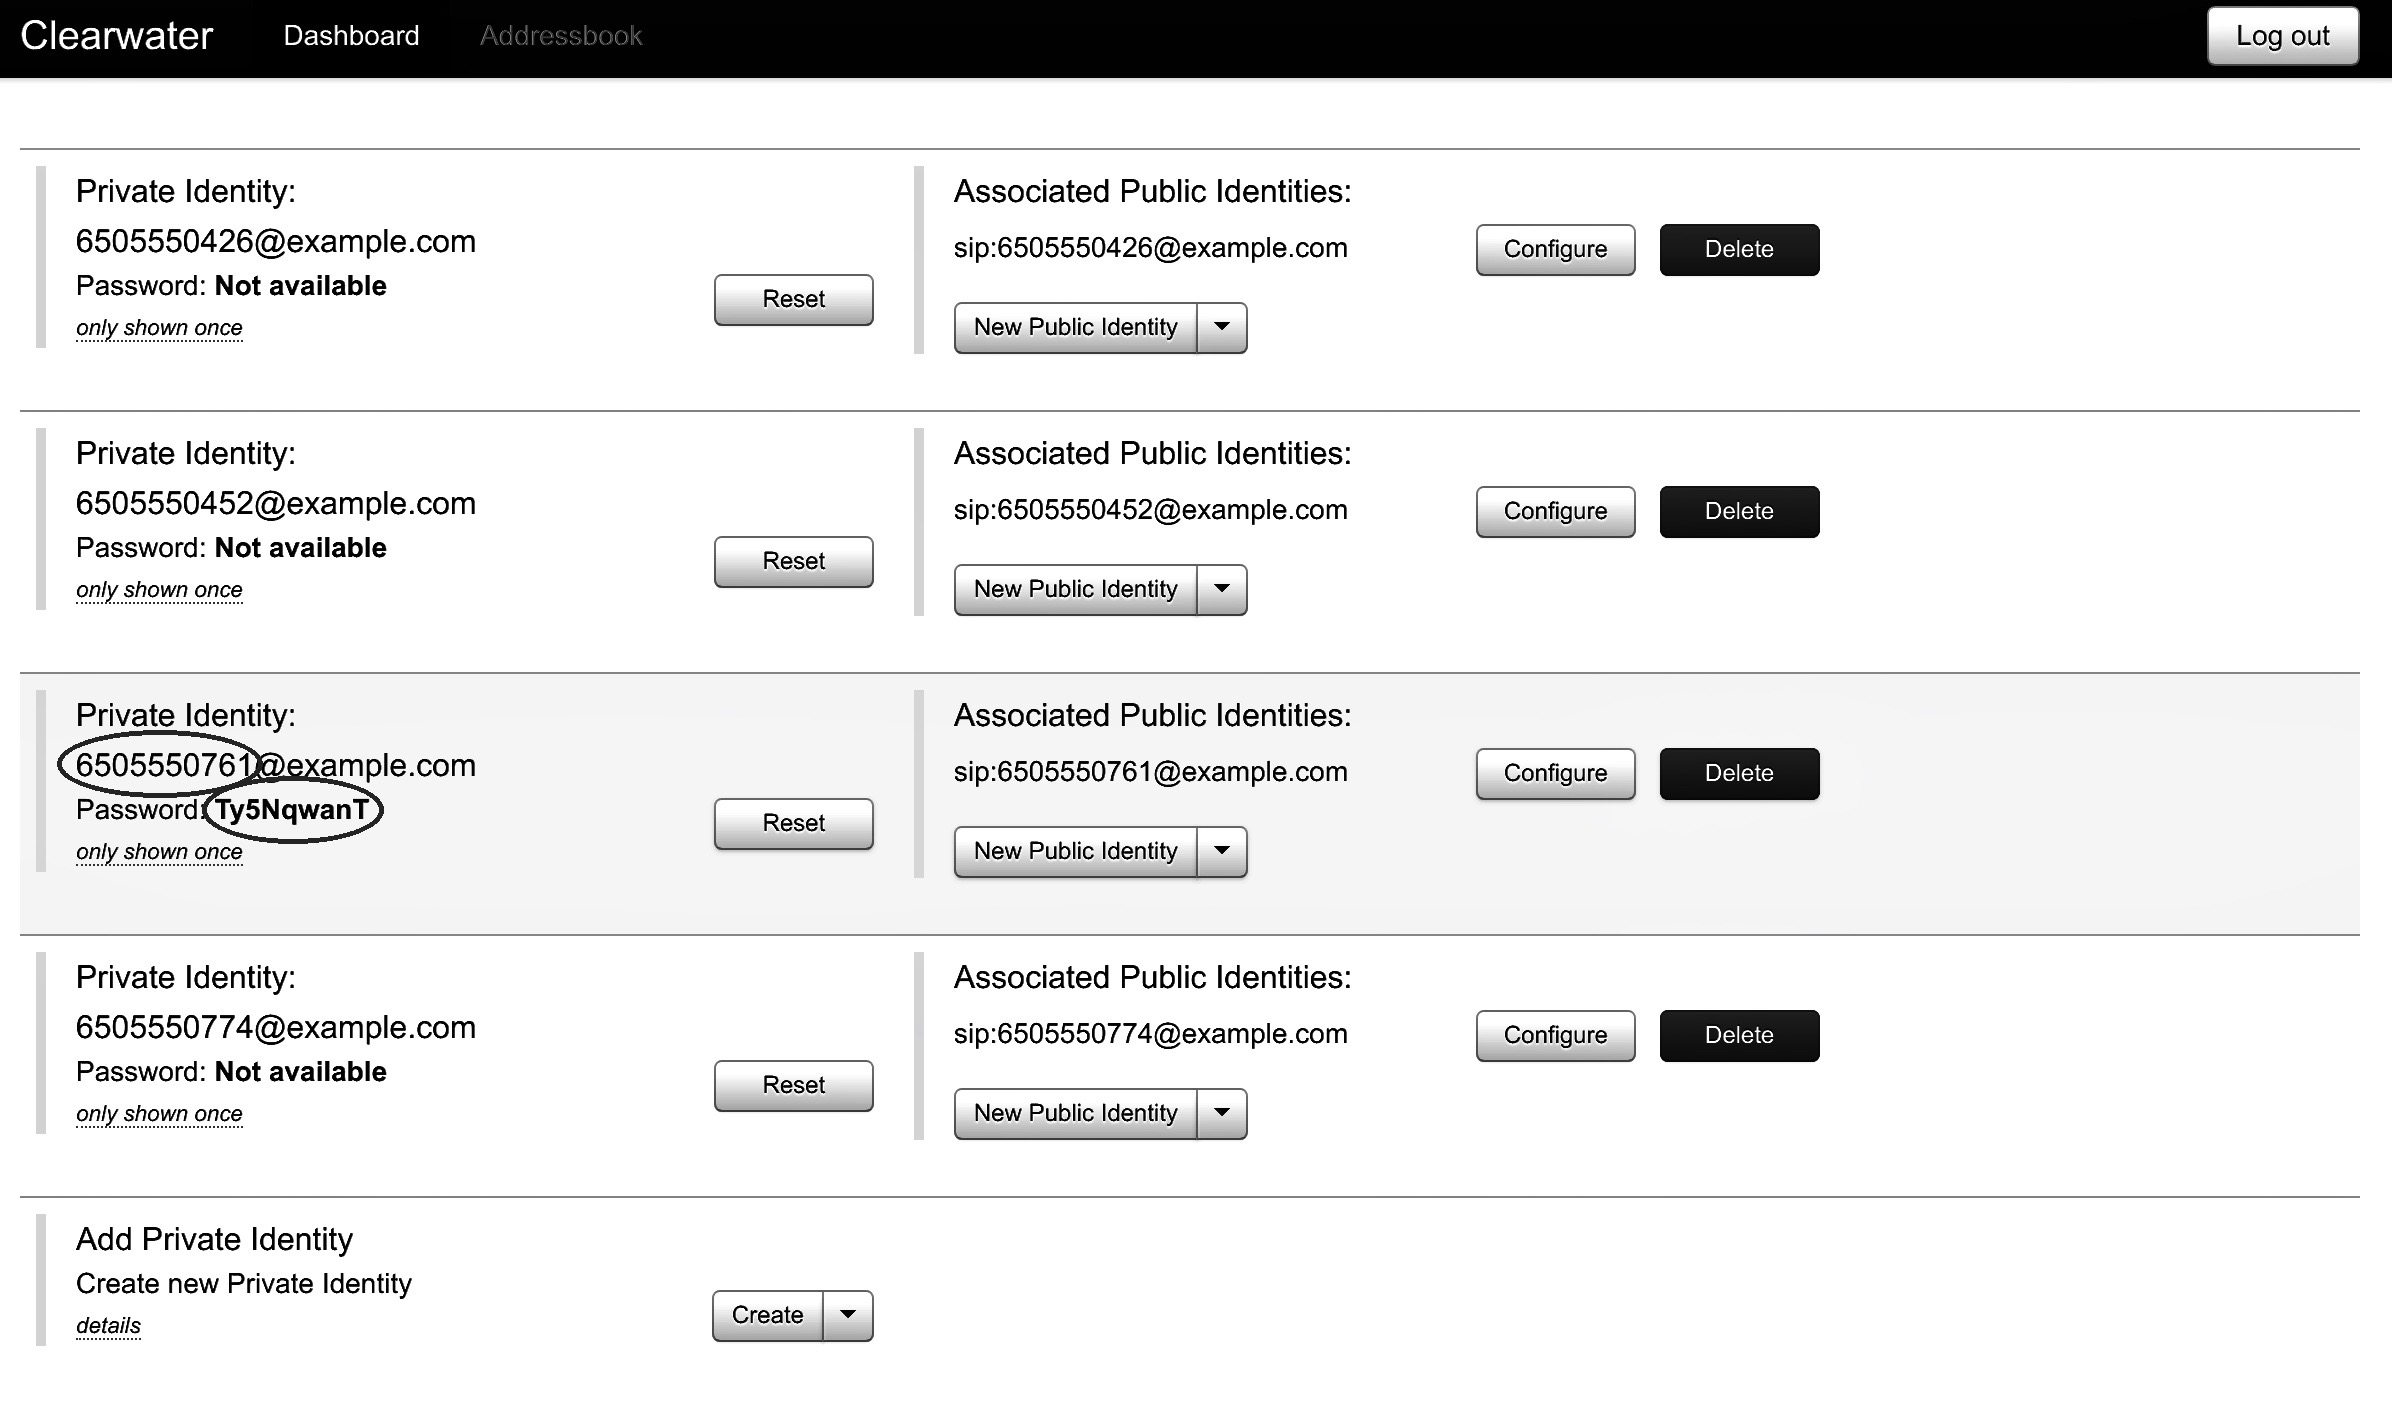
\includegraphics[width=\textwidth]{user}
\caption{مدیریت کاربران}
\label{user}
\end{figure}

در صفحه\nf ی مورد نظر، در قسمت \lr{Private Identity}، با کلیک بر روی گزینه \textbf{Create}، یک شماره تلفن جدید به فرمی مشابه آنچه در زیر می\nf بینید، ایجاد می\nf شود. قسمت \lr{6505551234} هم به عنوان نام\nf کاربری و هم به عنوان شماره تلفن کاربر استفاده می\nf شود. رمزعبور نیز در هنگام ثبت\nf نام \lr{SIP} استفاده می\nf شود. دقت شود که رمزعبور فقط یک بار نمایش داده می\nf شود و در دفعات بعدی که وارد این صفحه می\nf شوید، این رمز نشان داده نخواهدشد. با کلیک بر روی دکمه \textbf{Reset}، رمزعبور جدیدی برای شماره تلفن موردنظر ایجاد می\nf شود.

\begin{latin}
\setlength{\parindent}{0ex}
\noindent 6505551234@example.com\\
\noindent Password: 3At7dH5Md
\end{latin}

\section{پیکربندی  دستگاه کاربران}
\label{zoiperconf}

پس از ایجاد شماره تلفن برای کاربر، باید یک اپلیکیشن SIP روی دستگاه کاربر (تلفن همراه، رایانه شخصی و ...) نصب و سپس به\nf طور مناسب، پیکربندی شود. به دلایل خاصي، اگر این نوع پیاده\nf سازی روی سکّوی مجازی\nf سازی Virtualbox انجام شده باشد، حتماً باید یکی از طرفین مکالمه از اپلیکیشن zoiper استفاده کند. در این قسمت، برای سهولت کار فقط پیکربندی اپلیکیشن zoiper به همراه جزئیات توضیح داده شده است؛ بدیهی است که پیکربندی سایر اپلیکیشن\nf ها نیز مشابه همین روش خواهدبود. همچنین، سیستم میزبان و دستگاه کاربران همگی باید به آدرس IP یکدیگر دسترسی داشته باشند؛ یعنی بتوانند از طریق پروتکل \lr{IP}، با یکدیگر ارتباط برقرار کنند.

پس از نصب برنامه zoiper ، وارد آن شده و از نوار بالای صفحه، گزینه \lr{\textbf{Config}} را انتخاب کنید. سپس وارد قسمت \lr{\textbf{Accounts}} شده و بر روی عبارت \lr{\textbf{Add account}} کلیک کنید. در پاسخ به پرسش \lr{Do you already have an account?} گزینه \textbf{Yes} را انتخاب کنید. در پنجره جدید،گزینه \lr{\textbf{configuration Manual}} را انتخاب کنید. در صفحه جدیدی که باز می\nf شود، از شما خواسته\nf می\nf شود که نوع حساب کاربری را انتخاب کنید. از آنجایی که clearwater از پروتکل SIP استفاده میکند، باید گزینه \textbf{SIP} را انتخاب کنید. با این کار، وارد بخش پیکربندی حساب کاربری می\nf شوید.
 
در صفحه\nf ی پیکربندی حساب کاربری، روی گزینه\nf ی \textbf{name Account} کلیک کرده و یک نام دلخواه برای خود انتخاب کنید. سپس روی گزینه \textbf{Host} کلیک کرده و عبارت \textcolor{black}{'example.com'} را وارد کنید. در قسمت \textbf{Username} و \textbf{Password}، نام کاربری و رمز عبوری را که در قسمت ایجاد کاربر دریافت کرده\nf اید، وارد کنید. عبارت \textcolor{black}{example.com} را به \textcolor{black}{نام کاربری} خود اضافه کرده و در قسمت \textbf{user Authenticatoin} وارد کنید (به\nf عنوان مثال: \lr{6505551234@example.com}).

\begin{figure}[h]
\centering
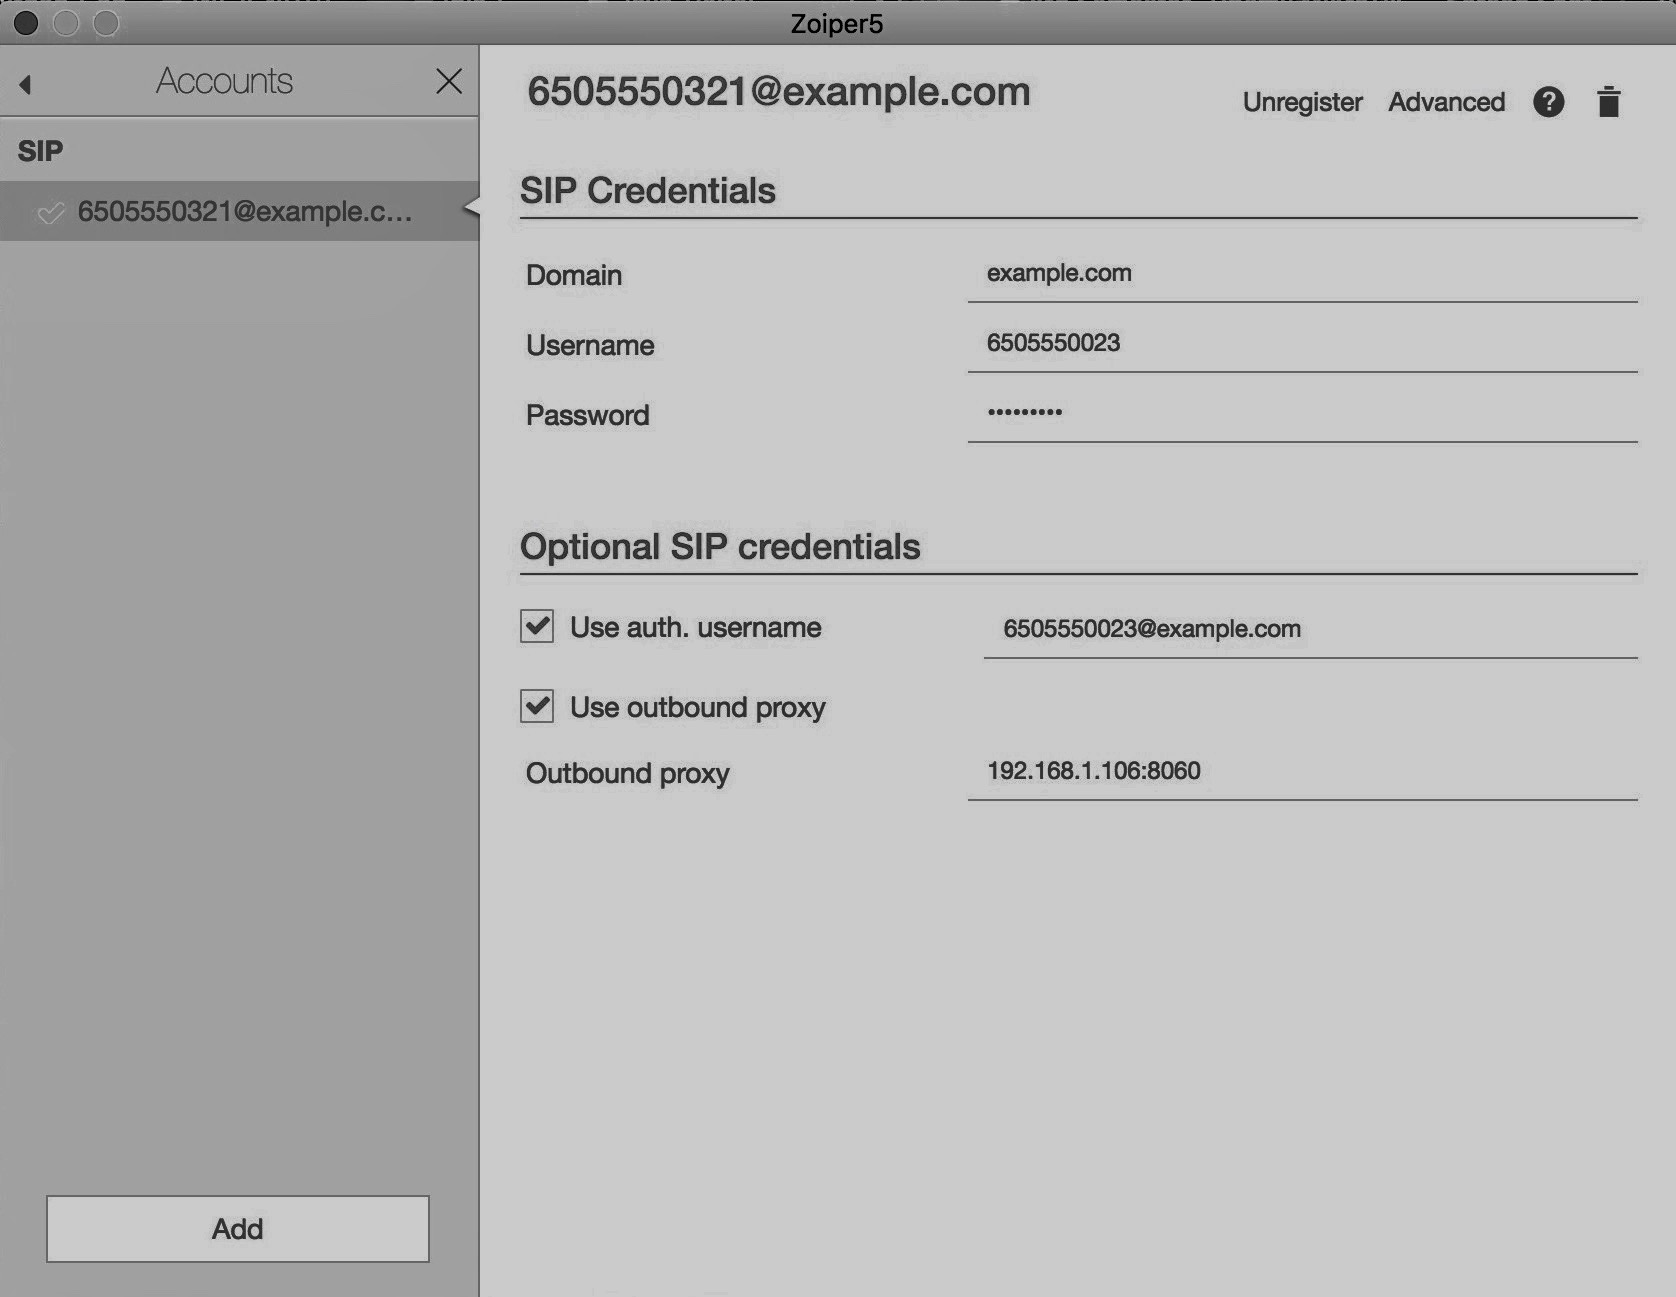
\includegraphics[width=0.7\textwidth]{zoiper}
\caption{صفحه\nf ی پیکربندی حساب کاربری در نسخه\nf ی دسکتاپ اپلیکیشن \lr{zoiper}}
\label{zoiperpic}
\end{figure}


پیکربندی انجام\nf شده تا این قسمت، مربوط به ورود اطّلاعات کاربر است. اکنون باید تنظیمات مربوط به شبکه انجام شود. آدرس IP ماشین میزبان خود را به دست\nf آورید. این آدرس را به همرا شماره پورت \lr{8060}، در قسمت \textbf{proxy Ountbound} وارد کنید. به عنوان مثال، اگر آدرس IP ماشین میزبان، \lr{192.168.1.30} است، شما باید عبارت \lr{192.168.1.30:8060} را در قسمت مذکور وارد کنید. سپس گزینه\nf ی \textbf{Setting Network} را انتخاب کنید. مطمئن شوید که \textbf{type Transport} از نوع \textcolor{black}{TCP} باشد. همچنین، \textbf{signalling for RPORT Use} باید \textcolor{black}{فعّال} باشد. قسمت \textbf{STUN Use} را نیز \textcolor{black}{غیر فعّال} کنید.

پس از انجام مراحل فوق، از قسمت مربوط به تنظیمات شبکه خارج شوید و سپس گزینه\nf ی \textbf{Save} را انتخاب کنید. اکنون، مراحل فوق را برای یک کاربر دیگر (با شماره تلفن متفاوت) انجام دهید. از آنجایی\nf که اپلیکیشن \lr{zoiper}، قابل نصب بر روی سیستم عامل\nf های مختلف است، می\nf توانید یک نسخه\nf ی مربوط به رایانه\nf ی شخصی(شکل \ref{zoiperpic}) خود را دریافت کرده و از طریق رایانه شخصی نیز تماس تلفنی برقرار کنید.



\section{برقراری تماس}
پس از ذخیره تنظیمات و پیکربندی\nf ها در مرحله قبل، اپلیکیشن به\nf طور خودکار عمل ثبت\nf نام را انجام می\nf دهد. پس از انجام مراحل فوق، هرگاه که کاربر به شبکه\nf ای متّصل شود که از طریق آن به IP ماشین میزبان دسترسی داشته باشد، اپلیکیشن \lr{zoiper} به\nf طور خودکار عملیّات ثبت\nf نام را انجام می\nf دهد. پس از انجام ثبت\nf نام، کاربر می\nf تواند با شماره\nf گیری سایر مشترکان این سیستم، با آن\nf ها تماس تلفنی برقرار کند(شماره\nf گیری باید در قسمت \lr{dialer} اپلیکیشن \lr{zoiper} انجام شود). این تماس تلفنی، از طریق هسته IMS و بر روی IP شکل می\nf گیرد و کیفیّت بالایی دارد. شکل \ref{cwtopo}، توپولوژی پیاده\nf سازی\nf شده برای راه\nf اندازی \lr{IMS} و برقراری تماس تلفنی بین کاربر تلفن همراه و کاربر رایانه\nf ی شخصی را نشان می\nf دهد.  در این پروژه تماس تلفنی از طریق \lr{IMS} بین دو کاربر تلفن همراه، بین دو کاربر رایانه\nf ی شخصی و همچنین بین کاربر تلفن همراه و کاربر رایانه\nf ی شخصی برقرار شد.

\begin{figure}[H]
\centering
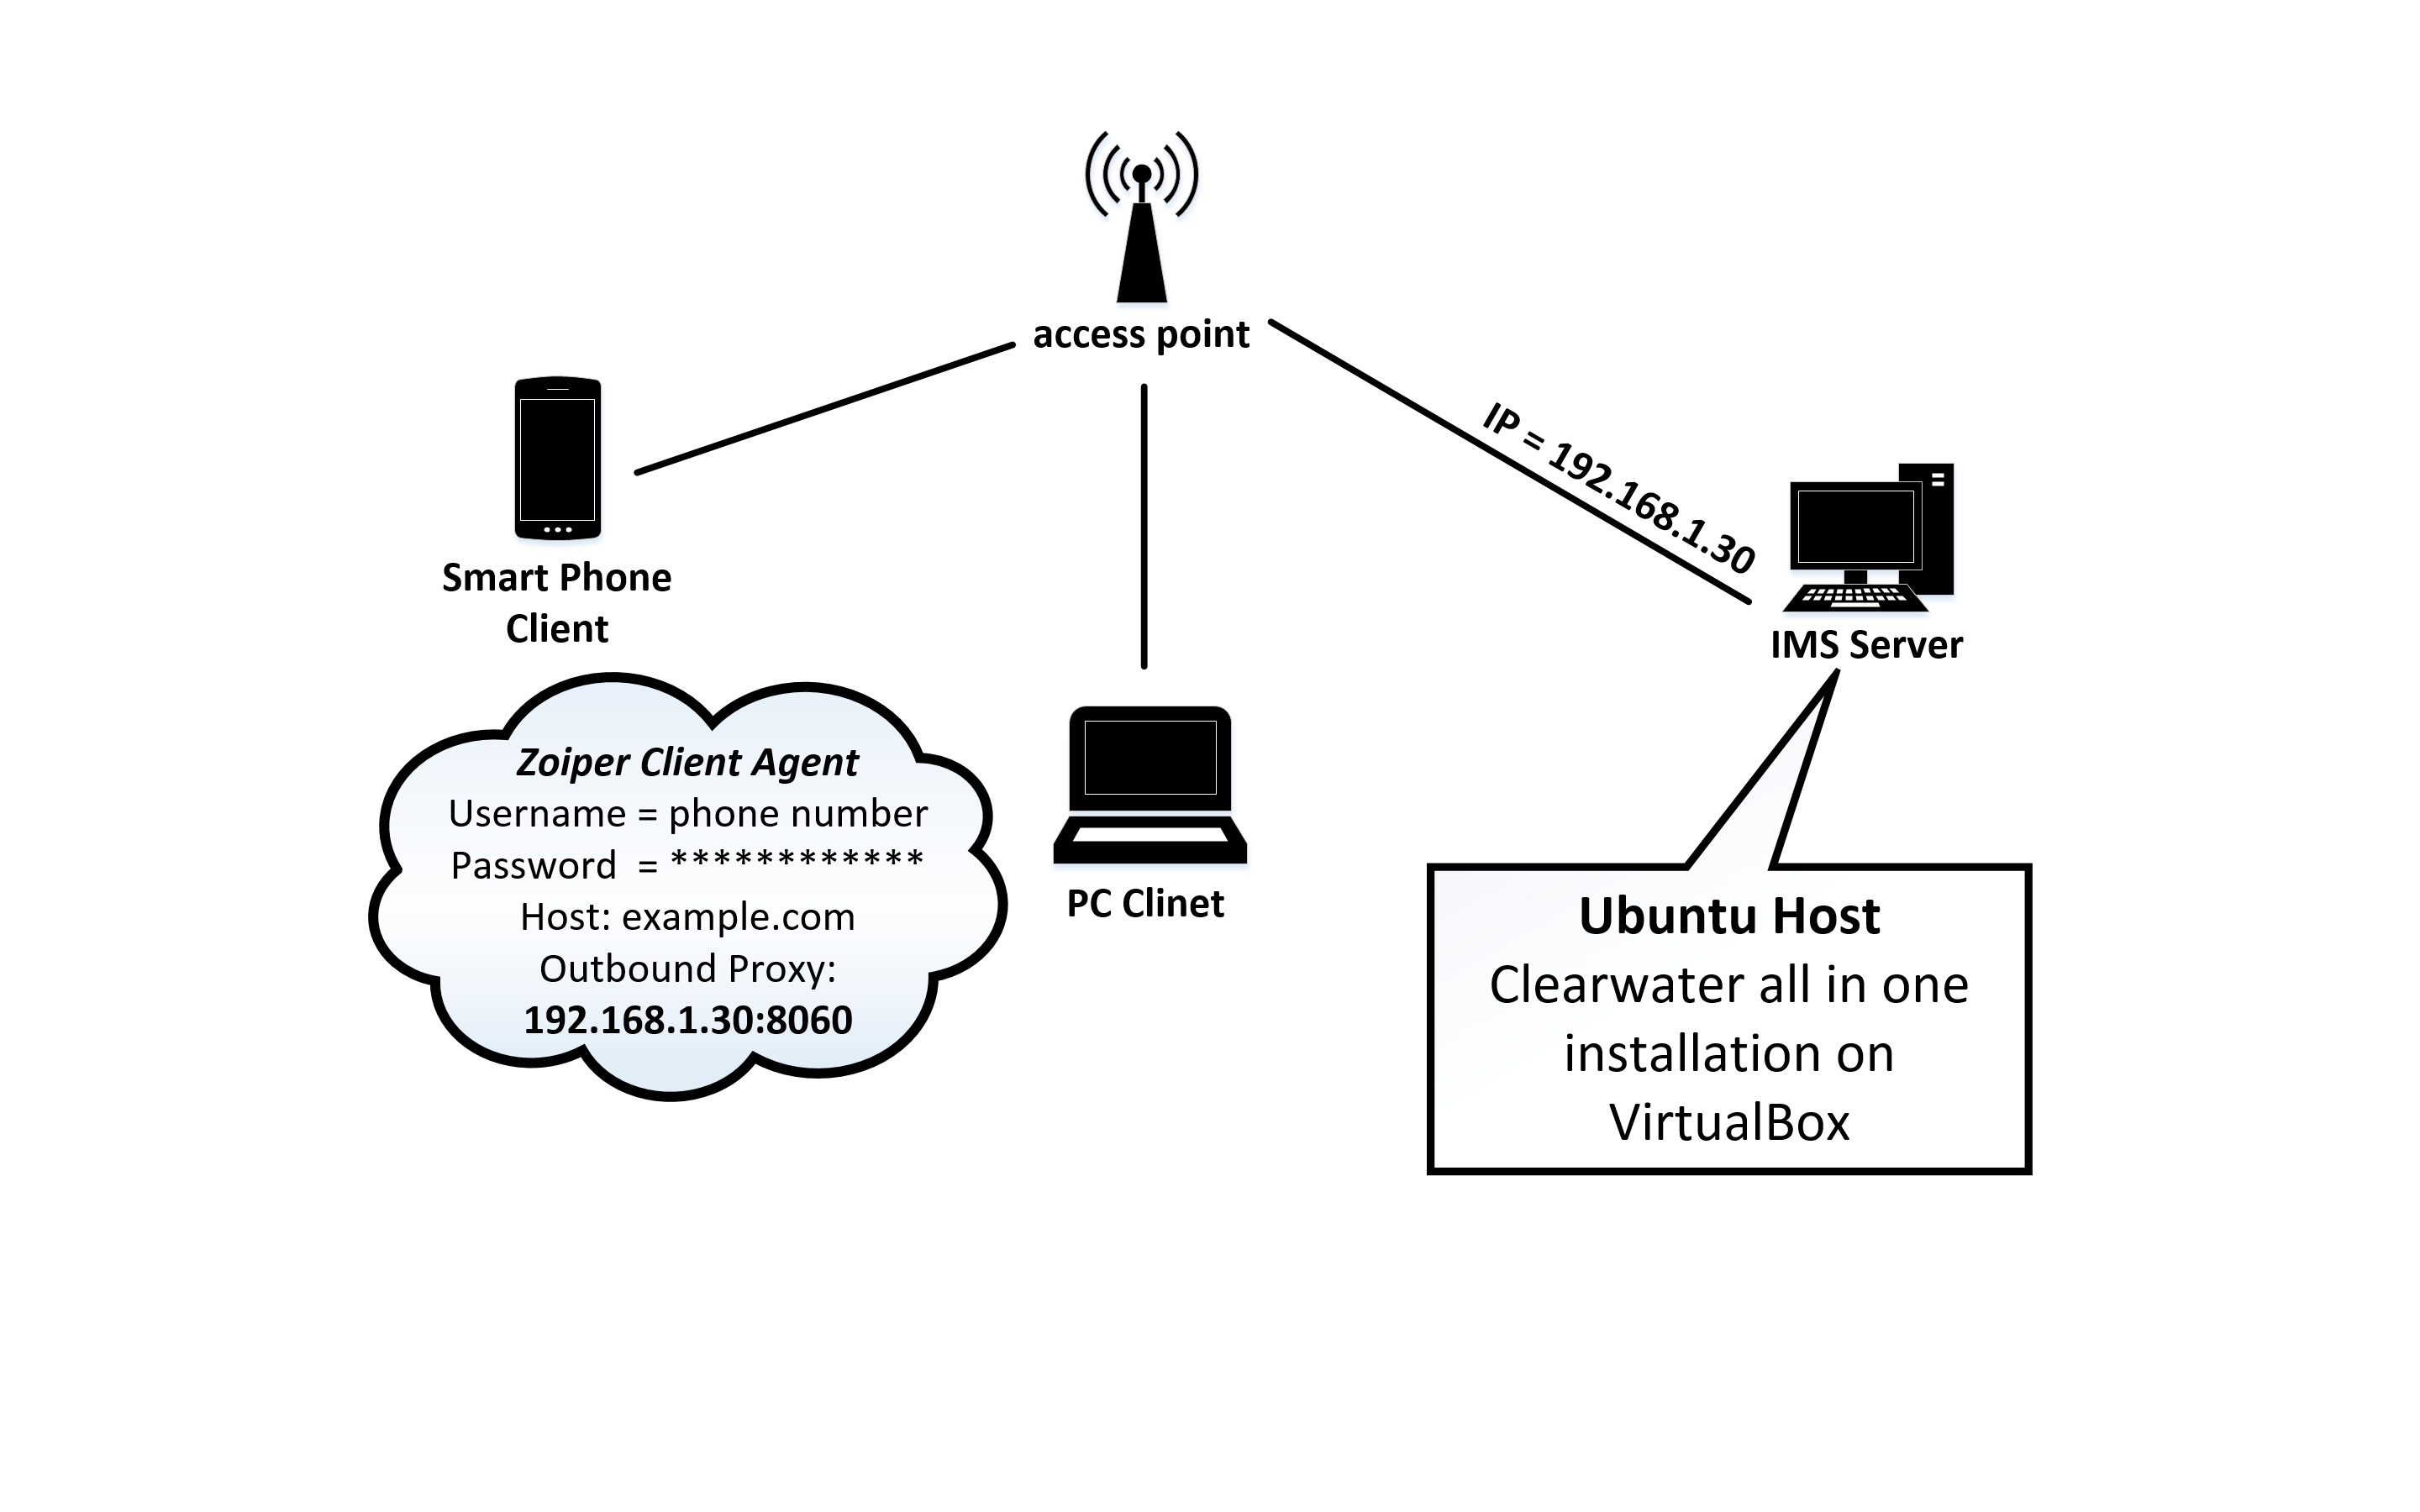
\includegraphics[width=0.68\textwidth]{cwaiotopo}
\caption{توپولوژی مورد استفاده برای برقراری تماس تلفنی از طریق \lr{IMS}}
\label{cwtopo}
\end{figure}

\section{آزمایش \lr{clearwater}}
\label{livetestPart}

روش\nf های گوناگونی برای آزمایش پیاده\nf سازی \lr{IMS}، توسّط \lr{clearwater} معرّفی شده\nf اند. یکی از این روش\nf ها، آزمایش زنده\RTLfootnote{\lr{Live Test}} است. آزمایش زنده را می\nf توان به\nf راحتی و به\nf صورت منظّم روی پیاده\nf سازی خود به اجرا درآورد تا بتوان از عملکرد صحیح کارکردهای سطح بالای سیستم\RTLfootnote{\lr{High level functoins}}، اطمینان حاصل کرد.

\subsubsection{نصب وابستگی\nf ها}
برای اجرای این آزمایش، نیاز است که نسخه \lr{1.9.3} زبان \lr{Ruby} بر روی ماشین مجازی \lr{clearwater} نصب شده باشد. برای انجام این فرایند، دستورات زیر را به ترتیب اجرا کنید.  در صورت عدم اجرای موفقیّت\nf آمیز هر یک از این دستورات، به پیوست (\ref{LiveTestA}) مراجعه شود.

\begin{latin}
\setlength{\parindent}{0ex}
1. sudo apt-get install build-essential git  -\nf -yes\\
2. curl -L http://get.rvm.io | bash -s stable\\
3. source \char`\~/.rvm/scripts/rvm\\
4. rvm autolibs enable\\
5. rvm install 1.9.3\\
6. rvm use 1.9.3\\
\end{latin}

\subsubsection{دانلود و نصب مجموعه برنامه\nf های  آزمایش \lr{clearwater} }

 ابتدا باید کلید \lr{ssh} برای برقراری ارتباط امن با \lr{github.com} در ماشین مجازی \lr{clearwater} وجود داشته باشد. برای بررسی وجود کلید \lr{ssh} و ساخت این کلید در صورت موجود نبودن آن، به \cite{gitssh} مراجعه شود. پس از ایجاد کلید \lr{ssh}، دستورات زیر باید به ترتیب اجرا شوند. این دستورات، مجموعه برنامه\nf های آزمایش \lr{clearwater} را دانلود و بر روی سیستم نصب می\nf کند. در صورت عدم اجرای موفقیّت\nf آمیز هر یک از دستورات زیر، به پیوست (\ref{LiveTestA}) مراجعه شود.
\begin{latin}
\setlength{\parindent}{0ex}
7. git clone -b stable -\nf -recursive git@github.com:Metaswitch/clearwater-live-test.git\\
8. cd clearwater-live-test\\
9. bundle install
\end{latin}

\subsubsection{اجرای آزمایش روی پیاده\nf سازی یکپارچه}
برای اجرای آزمایش زنده\nf ی \lr{clearwater}، دستور شماره \lr{10} را در خط فرمان ماشین مجازی \lr{clearwater} اجرا کنید. در این دستور، به\nf جای عبارت \lr{<code>} باید  \textbf{\lr{signup code}} سیستم قرار گیرد. این کد به صورت پیش\nf فرض، عبارت \textcolor{black}{'secret'} است. در صورتی که از پیاده\nf سازی بر روی سکّوی مجازی\nf سازی به روش خودکار استفاده شده است، به\nf جای عبارت \lr{<aio-identity>}، باید آدرس \lr{IP} ماشین مجازی قرار گیرد. این آدرس \lr{IP} که توسّط \lr{DHCP} به ماشین مجازی اختصاص داده شده است، آدرس آداپتور شبکه\nf ی\RTLfootnote{\lr{Network Adaptor}} ماشین مجازی است که روی حالت \lr{NAT} تنظیم شده است. این آدرس را می\nf توان با اجرای دستور \textbf{\lr{ifconfig}} و یا دستور \textbf{\lr{hostname -I}} روی ماشین مجازی، مشاهده نمود. خروجی اجرای تست، مانند شکل \ref{livetestpic} خواهدبود.
\begin{latin}
\setlength{\parindent}{0ex}
10. rake test[example.com] SIGNUP\_ CODE=<code> PROXY=<aio-identity> ELLIS=<aio-identity>
\end{latin}

\begin{figure}[H]
\centering
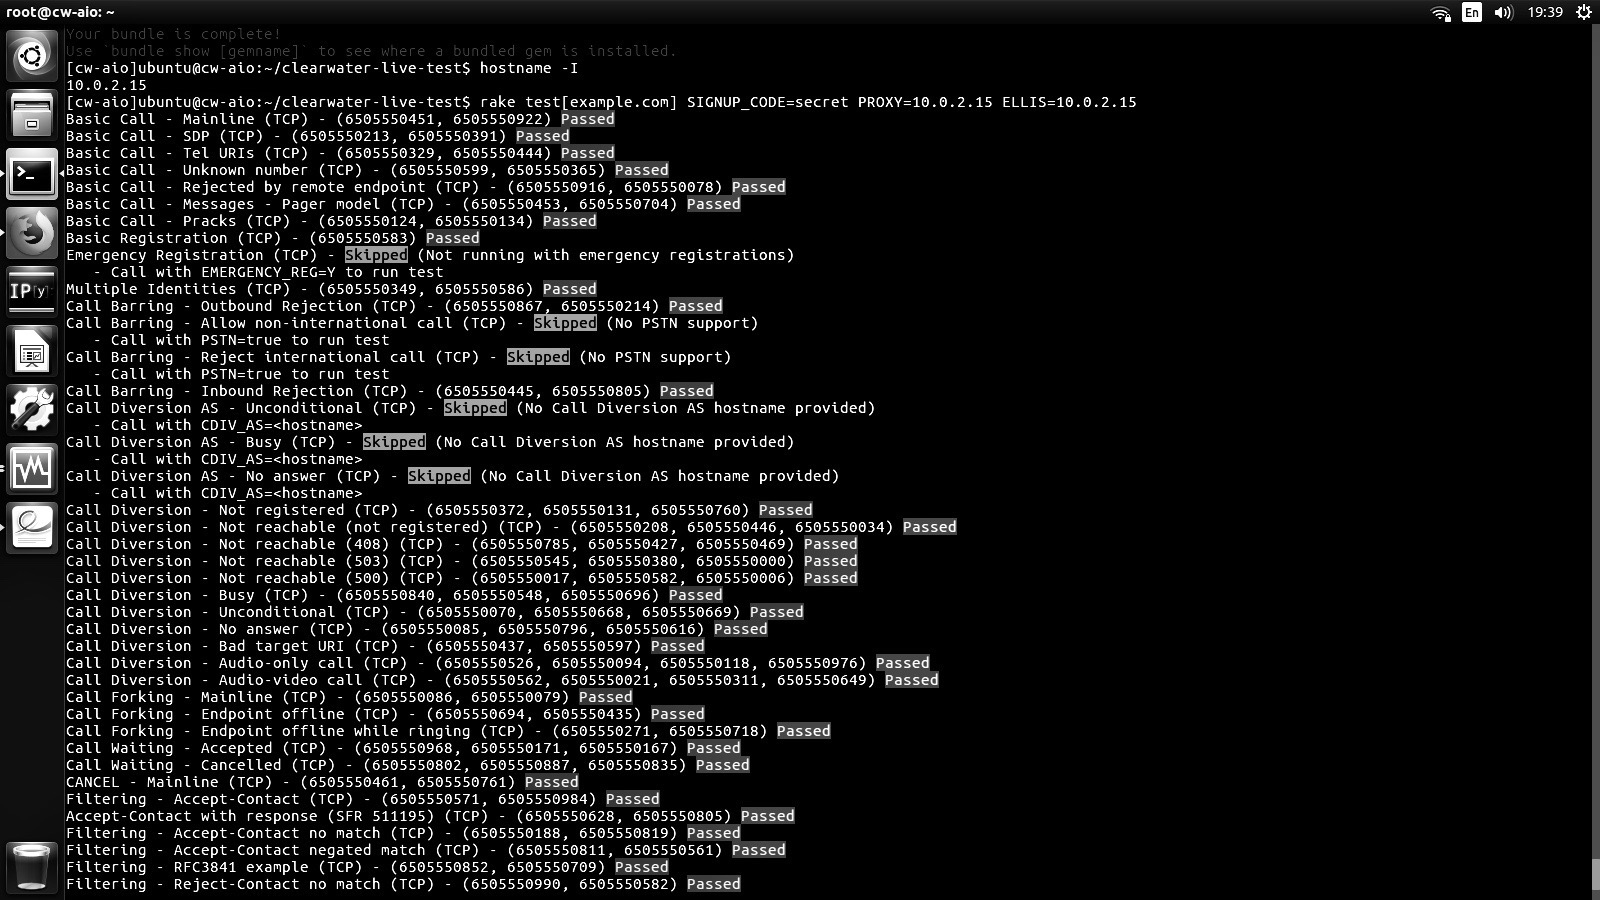
\includegraphics[width=\textwidth]{test}
\caption{خروجی اجرای آزمایش زنده\nf ی \lr{clearwater}}
\label{livetestpic}
\end{figure}